\documentclass{beamer}
\usetheme{Warsaw}
\usepackage{polski}
\usepackage[utf8]{inputenc}
\usepackage{verbatim}
\usepackage{graphicx}
\title
{Octopus}
\subtitle{multiplayer, casual, 2D shooter}
\author[]
{Bujok Mikołaj \and Kubiak Jakub \\ \and Szymon Miękus\and Nikodem Adrian}
\date[\today]
{Projekt zespołowy 2013}
\subject{Informatyka}

\begin{document}
%first frame
\frame{\titlepage}
\begin{frame}
  \frametitle{Agenda}
  \begin{itemize}
  \item O grze
  \item Architektura
  \item Narzędzia wspierania pracy
  \item Q\&A
  \end{itemize}
\end{frame}

% frame
\begin{frame}
  \frametitle{O grze}
  \begin{itemize}
    \item Reguły są proste - dwu wymiarowy DeathMatch
    \item Drużyny zaczynają na przeciwległych końcach mapy
    \item Mapy są symetryczne - zapewnia to zbalansowanie
          szans na poziomie architektury gry
    \item Na mapie losowo pojawiają się bonusy (chwilowe przyspieszanie, lepsza broń itp.
    \item Wygrywa ta drużna, która 'pozbędzie się' wszystkich przeciwników
  \end{itemize}
\end{frame}

% frame
\begin{frame}
\begin{figure}[ht]
\frametitle{O grze}
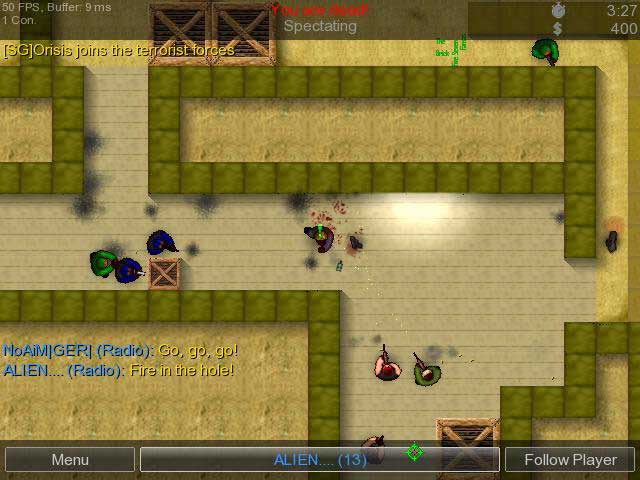
\includegraphics[scale=0.4]{cs2d.jpg}
\label{cs2d}
\caption{\href{http://www.unrealsoftware.de}{http://www.unrealsoftware.de}}
\end{figure}
\end{frame}
% frame
\begin{frame}

\frametitle{Architektura}
\begin{itemize}
\item Klient - Serwer
\item Obliczenia/przechowywanie stanu odbywa się na serwerze
\item Klient traktowany jako 'płótno' interpretujący dane z serwera i rysujący je
\item Serwer - Wielowątkową, zoptymalizowana maszyneria \\
 (made with secret alien technology)
\item Klient - Innowacyjna, responsywna, wykorzystująca HTML5 aplikacja, działająca wszędzie
tam gdzie można uruchomić przeglądarkę
\end{itemize}

\begin{figure}
   \centering
      
\includegraphics[scale=0.2]{lisp}
      
\includegraphics[scale=0.125]{html5}
\end{figure}
\end{frame}

\begin{frame}
\frametitle{Narzędzia wspierania pracy}
\begin{itemize}
\item Trello - jako oprogramowanie do zarządzania projektem \\
  \href{https://trello.com/}{https://trello.com/}
\item GitHub - jako platforma współpracy nad kodem \\
  \href{https://github.com}{https://github.com}
\item Git - jako system kontroli wersji \\
  \href{http://git-scm.com/}{http://git-scm.com/}
\end{itemize}
\end{frame}

\begin{frame}
\frametitle{Q\&A}
\end{frame}

\end{document}
